%%%%%%%%%%%%%%%%%%%%%%%%%%%%%%%%%%%%%%%%%%%%%%
%%
%%    D e s c r i p t i o n    o f     t h e      O b s e r v a t i o n s  : 
%%
%%%%%%%%%%%%%%%%%%%%%%%%%%%%%%%%%%%%%%%%%%%%%%
\noindent
After discussions with the MIRI Team (including European P.I.,
G. Wright and Instrument Scientist A. Glasse), we settled on the
strategy of picking one instrument (MIRI) and one observing mode
(MRS) and making sure we deliver the highest quality data analysis and
SEPs in this specific instance for the community. 

\smallskip \smallskip
\noindent
{\it Due to the nature of the ERS program, we note that we do not
necessarily have to observe a full, representative sample\footnote{Our
longer term goals will be to observe a representative sample of ERQs
across a range of redshifts to access e.g., the 9.7$\mu$m silicate
feature and 11.2, 12.7, and 16.4$\mu$m PAHs.} and given the
Discretionary time available for the ERS, a natural program size is
$\lesssim$35-40 hours.}  Moreover, our program specifically tests only
a particular mode of MIRI, albeit in detail, and thus our time request
is curtailed in that manner.  With these considerations in place, and
with the desire to immediately gain high signal-to-noise spectra in
order to investigate the physics and chemistry of quasar PAHs, along
with observational overhead concerns, pushes us to observe four
quasars, each object for 3.59 hours, for a total program Charged Time
of 22.20 hours.  The details of our four primary quasar targets are
given in Table~\ref{tab:targets}.


\begin{table}[h]
\begin{center}
\begin{tabular}{||  l|l|l|l|l ||}
  \hline\hline
  &&&& \\
  Object Name (SDSS)        & J0834+0159         &  J1232+0912          & J2215-0056        & J2323-0100 \\
  &&&& \\
  \hline
  &&&& \\
  Object R.A.                                & 08:34:48.48         & 12:32:41.73           & 22:15:24.00          & 23:23:26.17     \\
  object declination                     & $+$01:59:21.1     & $+$09:12:09.3      & $-$00:56:43.8      & $-$01:00:33.1  \\
  $r$-band AB magnitude            & 21.19$\pm$0.05  & 21.11$\pm$ 0.05  & 22.27$\pm$0.12  & 21.62$\pm$ 0.08 \\  
  WISE W4-band Vega magnitude & 6.88$\pm$0.09  & 6.78 $\pm$0.09   & 7.91$\pm$0.24  & 7.76$\pm$0.22 \\  
  WISE W4-band flux, $F_{\nu}$     & 14.80 mJy             & 16.23 mJy              & 5.73 mJy                 & 6.58 mJy  \\ 
  $i_{\rm AB}-W3_{\rm AB}$               & 6.0                        & 6.8                        & 6.2                        & 7.2\\
  Redshift $z$                               &  2.591                   &  2.381                    &  2.509                  &  2.356 \\  
  &&&& \\
  REW \civ                                 & 209$\pm$6          & 225$\pm$3          &153$\pm$5           &  256$\pm$5\\  
  \civ\ FWHM km s$^{-1}$          & 2863$\pm$65       & 4787$\pm$52       & 4280$\pm$112   & 3989$\pm$62 \\ 
  \oiii\ FWHM km s$^{-1}$       & 2811                      & 4971                     & 3057                    & 2625 \\ %% From Zam16
  % \oiii FWHM erg(??) s$^{-1}$ & ---                        & 5627                  & 3057                   & 2625 \\ %% From AlexandroffThesis
  &&&& \\
  ALMA  Band 6                  & {\it pending}                        & $\surd$                & {\it pending}                    & $\surd$  \\
  {\it HST} Cycle 24  ACS+WFC3     & obtained  &  {\it pending}   &{\it pending}  & {\it pending} \\
  Spectro-polarimertry       &   $\times$            &  $\surd$                &  $\surd$           & $\times$  \\
%  VLA data                          & ?                            &?                             & ?                        & ?  \\ 
 &&&& \\
Groups/Integrations/Exposures      &  45/1/1              &   15/3/1  &   45/1/1         &   15/3/1         \\
JWST target visibility (Start) & 2019-04-01    & 2019-05-08    & 2019-05-22   & 2019-06-07  \\ 
JWST target visibility (End)  & 2019-05-07    & 2019-07-01     & 2019-07-15   & 2019-07-29   \\ 
 &&&& \\
\hline\hline
      \end{tabular}
\caption{
Our four Extremely Red Quasar targets. All four quasars were first
identified in Ross et al. (2015).  Values of Rest Equivalent Widths
(REW) and Full Width Half Maxima (FWHM) are from Zakamska et
al. (2016) and Hamann et al. (2017).
}
\label{tab:targets} 
  \end{center}
\end{table}

%%\section*{MIRI MRS Observing Details}
%\vspace{-8pt}
%\smallskip \smallskip
\noindent
For our MIRI MRS operations we shall: 
\begin{itemize}
    \item Operate over the full spectral coverage, and thus will use all three different spectral settings;  
      SHORT (A), MEDIUM (B), and LONG (C). 
    \item Use the point source optimized, ``4-point ALL'' dither pattern.
      This is the only MIRI MRS dither patterns that guarantees ``GOOD''
      (i.e. half-integer) sampling throughout the common field of view
      across all four channels.
    \item{Detector Readout mode: SLOW. 
        Our integrations are relatively long, and the `Slow' mode readout pattern offers fewer detector
        artifacts and slightly lower detector noise than the `Fast' mode,  
        making it a good choice for faint source medium-resolution
        spectroscopy where the sky backgrounds are low. 
        This is what we want for our ERQ observations.}
\end{itemize}
We are interested in only a single object per point, so no mosaicking is necessary.  
The Subarray is FULL (this setting is fixed for MRS). 

\smallskip \smallskip
\noindent 
We desire high signal-to-noise in order to {\it(i)} detect any low
Equivalent Width PAH or AGN emission lines that might be resolved at
MRS resolutions and {\it(ii)} immediately compare our science results
to those of the {\it Spitzer Space Telescope} IRS studies.  {\it
With only 4 high-SNR JWST objects, we will have similar SNR as the
Spitzer IRS composite studies of $\gg100$ objects, and at similar
resolution.}  Long integrations also minimize Observatory overhead, a
desire that has been imparted on us by STScI operations.

\begin{figure}[h]
  \begin{center}
    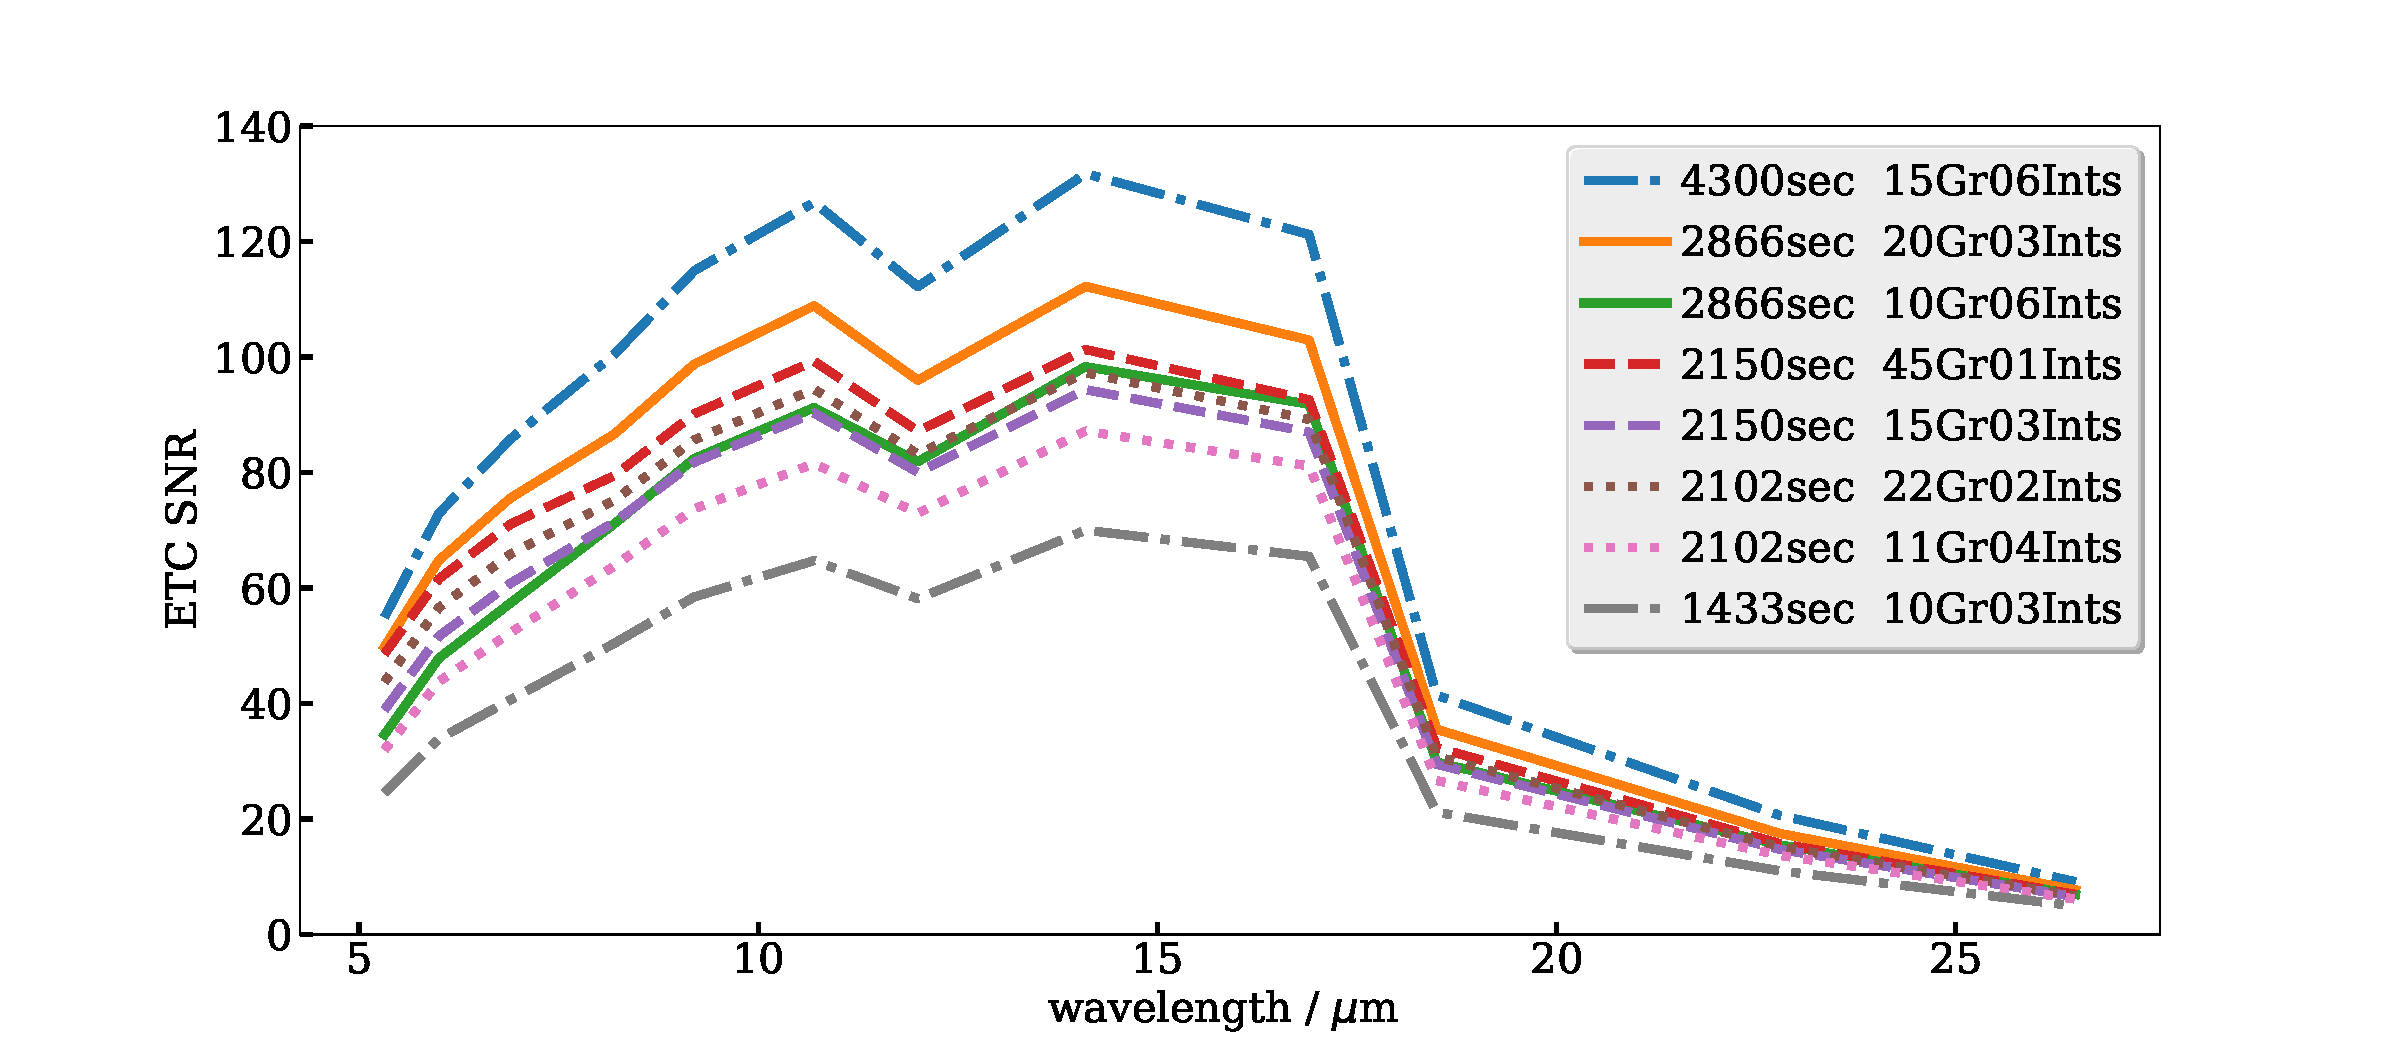
\includegraphics[height=7.0cm,width=16.5cm]{../ETC_calcs/SNR_vs_wavelength_comparisons_full.pdf}
    \end{center}
    \vspace{-20pt}
    \caption{ETC calculations of MIRI MRS SNR values for a range of Group
      sizes, Integrations and the associated Science exposure time (per
      Wavelength disperser). The SNR is from the ETC and is per pixel. 
      This exposure time 
      has to be multiplied by 24 to get the full Science Exposure time:   
      (a factor of 2 from the 2point in the ETC to 4-point dither; 
      a factor of 3 since for all three SHORT, MEDIUM and LONG modes and 
      a factor of 4 for the four quasars). 
 }
    \label{fig:SNR_vs_wavelength}
  \end{figure}

\smallskip \smallskip
\noindent 
For the observations themselves, a wide range of considerations e.g.,
sample size, desired high SNR, time available for ERS programs, level
of read noise, novelty of instrument, utility to the SEPs, etc., went
into our estimated time calculations.

\smallskip \smallskip 
\noindent
Our JWST ETC Workbook is
\href{https://jwst.etc.stsci.edu/workbook.html?wb_id=7474}{{\tt wb ID
7474}}.  In the ETC we assume the shape of the source is Point; a
Medium Background; the `IFU Nod In Scene'; Aperture location as
centered on source; an Aperture radius of 0.3''; Nod position in scene
of $X=Y=0.5''$.  We take the ``core ERQ'' SED that is given in Hamann
et al. (2017) and is fully representative of the ERQ population at
large.  The file
\href{https://github.com/d80b2t/JWST_ERS/blob/master/ETC_calcs/core_ERQ_SED_notLog.dat}{\tt
core\_ERQ\_SED\_notLog.dat} is used here.  We normalize this SED at a
wavelength of 23$\mu$m to a source flux density of 5mJy, again
representative (and if anything on the fainter end) of the WISE
W3/4-detected ERQ population and our targets.  At this stage we {\it
do not} include any emission (or absorption) lines since our null
hypothesis we want to test is that the IR emission is purely from an
AGN power-law.

\smallskip \smallskip 
\noindent
Figure~\ref{fig:SNR_vs_wavelength} shows our resulting SNR 
values for a range of Group, Integrations and Exposures. 
We ultimately decided to go with two combinations of the
Groups/Integrations/Exposures, for the same total Science Exposure
time; see~Table~\ref{tab:targets}.  
Our final observing time request is 3.59 hours Science exposure hours 
per object for 14.35 Science hours total. 
{\it Using Smart Accounting, the total Charged Time is 22.20 hours.}

 
%\Huge \huge \LARGE \Large \large \normalsize (default) \small 
\footnotesize 
%\scriptsize \tiny
\begin{table}
  \begin{center}
    \footnotesize 
    \begin{tabular}{|| l | l  l ||}
      \hline \hline
      Object name, SDSS J  	& R.A. (J2000) & Decl (J2000) \\
      \hline
      J000610.67+121501.2 &     00:06:10.6778 &+12:15:01.274 \\
      J014111.13-031852.5 &     01:41:11.1369 & -03:18:52.567 \\
      J083200.20+161500.3  & 08:32:00.2000 & +16:15:00.300 \\
      J113721.46+142728.8 &     11:37:21.4663 & +14:27:28.879 \\
      J121704.70+023417.1 & 12:17:04.7013 & +02:34:17.151 \\
      J134254.45+093059.3 &     13:42:54.4591 & +09:30:59.396  \\
      J135608.32+073017.2 & 13:56:08.3200 & +07:30:17.200\\
      J162518.66+144509.9 &     16:25:18.6600 & +14:45:09.900 \\
      J215855.10-014717.9 &     21:58:55.1028& -01:47:17.973 \\
      J222307.12+085701.7 & 22:23:07.1253 & +08:57:01.735\\
      \hline\hline
    \end{tabular}
    \caption{A list of Secondary targets. All of these objects will
      have ALMA Cycle 5 Band 6 observations. Observations of these would
      allow us to achieve our SEP and Science goals.}
\label{tab:backups} 
\end{center}
\end{table}
\normalsize




